\documentclass[10pt]{article}
\usepackage[polish]{babel}
\usepackage[utf8]{inputenc}
\usepackage[T1]{fontenc}
\usepackage{amsmath}
\usepackage{amsfonts}
\usepackage{amssymb}
\usepackage[version=4]{mhchem}
\usepackage{stmaryrd}
\usepackage{graphicx}
\usepackage[export]{adjustbox}
\graphicspath{ {./images/} }

\title{Instrukcja dla zdającego }

\author{}
\date{}


\begin{document}
\maketitle
MATEMATYKA - poziom rozszerzony LO

Czas pracy:

\begin{enumerate}
  \item Sprawdź, czy arkusz egzaminacyjny zawiera 16 stron (zadania 1-16). Ewentualny brak zgłoś przewodniczącemu zespołu nadzorującego egzamin.
  \item Rozwiązania zadań i odpowiedzi wpisuj w miejscu na to przeznaczonym.
  \item Pamiętaj, że pominięcie argumentacji lub istotnych obliczeń w rozwiązaniu zadania otwartego może spowodować, że za to rozwiązanie nie otrzymasz pełnej liczby punktów.
  \item Pisz czytelnie i używaj tylko długopisu lub pióra z czarnym tuszem lub atramentem.
  \item Nie używaj korektora, a błędne zapisy wyraźnie przekreśl. Pamiętaj, że zapisy w brudnopisie nie będą oceniane.
  \item Możesz korzystać z zestawu wzorów matematycznych, cyrkla i linijki oraz kalkulatora prostego.
  \item Nie wpisuj żadnych znaków w części przeznaczonej dla egzaminatora.
\end{enumerate}

W zadaniach o numerach od 1 do 5 wybierz i zaznacz na karcie odpowiedzi jedną poprawną odpowiedź

\section*{Zadanie 1. (1pkt)}
Zbiorem wartości funkcji \(f(x)=\sqrt{-\sqrt{-x-4}}\) jest:\\
A. \(\{0\}\)\\
B. zbiór pusty\\
C. \((0,+\infty)\)\\
D. \((-\infty,-4)\)

Zadanie 2. (1pkt)\\
Dziedziną funkcji \(f(x)=\log _{2015}\left(\log _{\frac{1}{2015}}\left(\log _{2015} x\right)\right)\) jest zbiór:\\
A. \(x \in(215,+\infty)\)\\
B. \(x \in(1,2015)\)\\
C. \(x \in(0,+\infty)\)\\
D. \(x \in(0,2015)\)

Zadanie 3. ( \(1 p k t)\)\\
Okrąg o środku w punkcie \(\mathrm{S}(-1 ; 2)\) jest styczny do prostej o równaniu \(4 \mathrm{x}-3 \mathrm{y}+3=0\).\\
Promień okręgu jest równy :\\
A. \(\frac{2}{5}\)\\
B. 1\\
C. \(\frac{7}{5}\)\\
D. \(\sqrt{8}\)

Zadanie 4. (lpkt)\\
Wycinek kołowy o kącie środkowym \(120^{\circ}\) i polu \(3 \pi\) zwinięto w stożek. Promień podstawy tego stożka jest równy:\\
A. 2,5\\
B. 2\\
C. 1,6\\
D. 1

\section*{Zadanie 5. (lpkt)}
W czworościanie foremnym cosinus kąta dwuściennego między dwiema sąsiednimi ścianami jest równy:\\
A. 0\\
B. 0,25\\
C. \(\frac{1}{3}\)\\
D. \(\frac{1}{2}\)

\begin{center}
\begin{tabular}{|c|c|c|c|c|c|c|c|c|c|c|c|c|c|c|c|c|c|c|c|c|c|c|c|}
\hline
 &  &  &  &  &  &  &  &  &  &  &  &  &  &  &  &  &  &  &  &  &  &  &  \\
\hline
 &  &  &  &  &  &  &  &  &  &  &  &  &  &  &  &  &  &  &  &  &  &  &  \\
\hline
 &  &  &  &  &  &  &  &  &  &  &  &  &  &  &  &  &  &  &  &  &  &  &  \\
\hline
 &  &  &  &  &  &  &  &  &  &  &  &  &  &  &  &  &  &  &  &  &  &  &  \\
\hline
 &  &  &  &  &  &  &  &  &  &  &  &  &  &  &  &  &  &  &  &  &  &  &  \\
\hline
 &  &  &  &  &  &  &  &  &  &  &  &  &  &  &  &  &  &  &  &  &  &  &  \\
\hline
 &  &  &  &  &  &  &  &  &  &  &  &  &  &  &  &  &  &  &  &  &  &  &  \\
\hline
 &  &  &  &  &  &  &  &  &  &  &  &  &  &  &  &  &  &  &  &  &  &  &  \\
\hline
 &  &  &  &  &  &  &  &  &  &  &  &  &  &  &  &  &  &  &  &  &  &  &  \\
\hline
 &  &  &  &  &  &  &  &  &  &  &  &  &  &  &  &  &  &  &  &  &  &  &  \\
\hline
 &  &  &  &  &  &  &  &  &  &  &  &  &  &  &  &  &  &  &  &  &  &  &  \\
\hline
 &  &  &  &  &  &  &  &  &  &  &  &  &  &  &  &  &  &  &  &  &  &  &  \\
\hline
 &  &  &  &  &  &  &  &  &  &  &  &  &  &  &  &  &  &  &  &  &  &  &  \\
\hline
 &  &  &  &  &  &  &  &  &  &  &  &  &  &  &  &  &  &  &  &  &  &  &  \\
\hline
 &  &  &  &  &  &  &  &  &  &  &  &  &  &  &  &  &  &  &  &  &  &  &  \\
\hline
 &  &  &  &  &  &  &  &  &  &  &  &  &  &  &  &  &  &  &  &  &  &  &  \\
\hline
 &  &  &  &  &  &  &  &  &  &  &  &  &  &  &  &  &  &  &  &  &  &  &  \\
\hline
 &  &  &  &  &  &  &  &  &  &  &  &  &  &  &  &  &  &  &  &  &  &  &  \\
\hline
 &  &  &  &  &  &  &  &  &  &  &  &  &  &  &  &  &  &  &  &  &  &  &  \\
\hline
 &  &  &  &  &  &  &  &  &  &  &  &  &  &  &  &  &  &  &  &  &  &  &  \\
\hline
 &  &  &  &  &  &  &  &  &  &  &  &  &  &  &  &  &  &  &  &  &  &  &  \\
\hline
 &  &  &  &  &  &  &  &  &  &  &  &  &  &  &  &  &  &  &  &  &  &  &  \\
\hline
\end{tabular}
\end{center}

W zadaniu 6 zakoduj we wskazanym miejscu wynik zgodnie z poleceniem.

\section*{Zadanie 6. (2pkt)}
Oblicz: \(\quad \lim _{x \rightarrow 1} \frac{x^{3}-x^{2}+x-1}{2 x^{3}-2}\)\\
Zakoduj pierwsze trzy cyfry rozwinięcia dziesiętnego otrzymanego wyniku.

\begin{center}
\begin{tabular}{|l|l|l|}
\hline
dziesiąte & setne & tysiączne \\
\hline
 &  &  \\
\hline
\end{tabular}
\end{center}

\begin{center}

\includegraphics[max width=\textwidth]{2024_11_21_12a27a32a51fef2c834ag-04}
\end{center}

Rozwiązania zadań od 7 do 17. należy zapisać w wyznaczonych miejscach pod treścią zadania.

\section*{Zadanie 7. (3pkt)}
Udowodnij, że dla każdej liczby rzeczywistej x prawdziwa jest nierówność \(x^{4}-x^{2}-2 x+3>0\).

\begin{center}
\begin{tabular}{|c|c|c|c|c|c|c|c|c|c|c|c|c|c|c|c|c|c|c|c|c|c|c|c|c|c|c|c|c|c|c|}
\hline
 &  &  &  &  &  &  &  &  &  &  &  &  &  &  &  &  &  &  &  &  &  &  &  &  &  &  &  &  &  &  \\
\hline
 &  &  &  &  &  &  &  &  &  &  &  &  &  &  &  &  &  &  &  &  &  &  &  &  &  &  &  &  &  &  \\
\hline
 &  &  &  &  &  &  &  &  &  &  &  &  &  &  &  &  &  &  &  &  &  &  &  &  &  &  &  &  &  &  \\
\hline
 &  &  &  &  &  &  &  &  &  &  &  &  &  &  &  &  &  &  &  &  &  &  &  &  &  &  &  &  &  &  \\
\hline
 &  &  &  &  &  &  &  &  &  &  &  &  &  &  &  &  &  &  &  &  &  &  &  &  &  &  &  &  &  &  \\
\hline
 &  &  &  &  &  &  &  &  &  &  &  &  &  &  &  &  &  &  &  &  &  &  &  &  &  &  &  &  &  &  \\
\hline
 &  &  &  &  &  &  &  &  &  &  &  &  &  &  &  &  &  &  &  &  &  &  &  &  &  &  &  &  &  &  \\
\hline
 &  &  &  &  &  &  &  &  &  &  &  &  &  &  &  &  &  &  &  &  &  &  &  &  &  &  &  &  &  &  \\
\hline
 &  &  &  &  &  &  &  &  &  &  &  &  &  &  &  &  &  &  &  &  &  &  &  &  &  &  &  &  &  &  \\
\hline
 &  &  &  &  &  &  &  &  &  &  &  &  &  &  &  &  &  &  &  &  &  &  &  &  &  &  &  &  &  &  \\
\hline
 &  &  &  &  &  &  &  &  &  &  &  &  &  &  &  &  &  &  &  &  &  &  &  &  &  &  &  &  &  &  \\
\hline
 &  &  &  &  &  &  &  &  &  &  &  &  &  &  &  &  &  &  &  &  &  &  &  &  &  &  &  &  &  &  \\
\hline
 &  &  &  &  &  &  &  &  &  &  &  &  &  &  &  &  &  &  &  &  &  &  &  &  &  &  &  &  &  &  \\
\hline
 &  &  &  &  &  &  &  &  &  &  &  &  &  &  &  &  &  &  &  &  &  &  &  &  &  &  &  &  &  &  \\
\hline
 &  &  &  &  &  &  &  &  &  &  &  &  &  &  &  &  &  &  &  &  &  &  &  &  &  &  &  &  &  &  \\
\hline
 &  &  &  &  &  &  &  &  &  &  &  &  &  &  &  &  &  &  &  &  &  &  &  &  &  &  &  &  &  &  \\
\hline
 &  &  &  &  &  &  &  &  &  &  &  &  &  &  &  &  &  &  &  &  &  &  &  &  &  &  &  &  &  &  \\
\hline
 &  &  &  &  &  &  &  &  &  &  &  &  &  &  &  &  &  &  &  &  &  &  &  &  &  &  &  &  &  &  \\
\hline
 &  &  &  &  &  &  &  &  &  &  &  &  &  &  &  &  &  &  &  &  &  &  &  &  &  &  &  &  &  &  \\
\hline
 &  &  &  &  &  &  &  &  &  &  &  &  &  &  &  &  &  &  &  &  &  &  &  &  &  &  &  &  &  &  \\
\hline
 &  &  &  &  &  &  &  &  &  &  &  &  &  &  &  &  &  &  &  &  &  &  &  &  &  &  &  &  &  &  \\
\hline
 &  &  &  &  &  &  &  &  &  &  &  &  &  &  &  &  &  &  &  &  &  &  &  &  &  &  &  &  &  &  \\
\hline
 &  &  &  &  &  &  &  &  &  &  &  &  &  &  &  &  &  &  &  &  &  &  &  &  &  &  &  &  &  &  \\
\hline
 &  &  &  &  &  &  &  &  &  &  &  &  &  &  &  &  &  &  &  &  &  &  &  &  &  &  &  &  &  &  \\
\hline
 &  &  &  &  &  &  &  &  &  &  &  &  &  &  &  &  &  &  &  &  &  &  &  &  &  &  &  &  &  &  \\
\hline
 &  &  &  &  &  &  &  &  &  &  &  &  &  &  &  &  &  &  &  &  &  &  &  &  &  &  &  &  &  &  \\
\hline
 &  &  &  &  &  &  &  &  &  &  &  &  &  &  &  &  &  &  &  &  &  &  &  &  &  &  &  &  &  &  \\
\hline

\includegraphics[max width=\textwidth]{2024_11_21_12a27a32a51fef2c834ag-05}
 &  &  &  &  &  &  &  &  &  &  &  &  &  &  &  &  &  &  &  &  &  &  &  &  &  &  &  &  &  &  \\
\hline
 &  &  &  &  &  &  &  &  &  &  &  &  &  &  &  &  &  &  &  &  &  &  &  &  &  &  &  &  &  &  \\
\hline

\includegraphics[max width=\textwidth]{2024_11_21_12a27a32a51fef2c834ag-05(1)}
 &  &  &  &  &  &  &  &  &  &  &  &  &  &  &  &  &  &  &  &  &  &  &  &  &  &  &  &  &  &  \\
\hline
 &  &  &  &  &  &  &  &  &  &  &  &  &  &  &  &  &  &  &  &  &  &  &  &  &  &  &  &  &  &  \\
\hline
- &  &  &  &  &  &  &  &  &  &  &  &  &  &  &  &  &  &  &  &  &  &  &  &  &  &  &  &  &  &  \\
\hline
, &  &  &  &  &  &  &  &  &  &  &  &  &  &  &  &  &  &  &  &  &  &  &  &  &  &  &  &  &  &  \\
\hline
 &  &  &  &  &  &  &  &  &  &  &  &  &  &  &  &  &  &  &  &  &  &  &  &  &  &  &  &  &  &  \\
\hline
 & - &  &  &  &  &  &  &  &  &  &  &  &  &  &  &  &  &  &  &  &  &  &  &  &  &  &  &  &  &  \\
\hline
 &  &  &  &  &  &  &  &  &  &  &  &  &  &  &  &  &  &  &  &  &  &  &  &  &  &  &  &  &  &  \\
\hline
 &  &  &  &  &  &  &  &  &  &  &  &  &  &  &  &  &  &  &  &  &  &  &  &  &  &  &  &  &  &  \\
\hline
 &  &  &  &  &  &  &  &  &  &  &  &  &  &  &  &  &  &  &  &  &  &  &  &  &  &  &  &  &  &  \\
\hline
 &  &  &  &  &  &  &  &  &  &  &  &  &  &  &  &  &  &  &  &  &  &  &  &  &  &  &  &  &  &  \\
\hline
\end{tabular}
\end{center}

\section*{Zadanie 8. (4pkt)}
Rozwiąż równanie: \(x^{2}+2 x^{3}+4 x^{4}+\ldots \ldots=\lim _{n \rightarrow \infty} \frac{1-3 n}{2-9 n}\),\\
gdzie lewa strona równania jest sumą nieskończonego ciągu geometrycznego.

\section*{Zadanie 9. (4 pkt)}
Dla jakich wartości parametru \(k \in R\) równanie \(\sin ^{6} \alpha+\cos ^{6} \alpha=k\) ma rozwiązanie?

Zadanie 10. ( 4 p )\\
Oblicz pole trójkąta utworzonego przez osie układu współrzędnych i przez prostą o ujemnym współczynniku kierunkowym m do której należy punkt \(\mathrm{A}(1,1)\). Dla jakiej wartości m pole tego trójkąta jest najmniejsze?\\

\includegraphics[max width=\textwidth, center]{2024_11_21_12a27a32a51fef2c834ag-07}

Zadanie 11. ( 4p )\\
W pewnym przedsiębiorstwie 9\% wyrobów jest brakami. Na 100dobrych wyrobów 70 jest pierwszego gatunku. Jakie jest prawdopodobieństwo, że wylosowana sztuka jest pierwszego gatunku?\\

\includegraphics[max width=\textwidth, center]{2024_11_21_12a27a32a51fef2c834ag-08}

\section*{Zadanie 12. (4p)}
Wysokość podstawy graniastosłupa prawidłowego trójkątnego ma długość \(4 \sqrt{3}\), zaś przekątna ściany bocznej tworzy z krawędzią podstawy kąt równy \(\frac{\pi}{3}\). Graniastosłup ten wpisano w walec. Oblicz pole powierzchni i objętość walca.

Zadanie 13. (5p)\\
Dla jakich wartości parametru a równanie \(|x+a|=1-||x-2|-3|\) ma dokładnie 2 rozwiązania?

Zadanie 14. (5p )\\
Wyznacz równania wszystkich stycznych do wykresu funkcji \(f(x)=\frac{x}{1-x^{2}}, \quad x \in R-\{-1,1\}\) nachylonych do osi Ox pod kątem \(45^{\circ}\).\\

\includegraphics[max width=\textwidth, center]{2024_11_21_12a27a32a51fef2c834ag-11}

Zadanie 15. (5p )\\
Dany jest wielomian \(W(x)=x^{5}-x^{4}+n x^{3}+k x+m\).\\
Wyznacz wszystkie wartości parametrów \(\mathrm{n}, \mathrm{k}, \mathrm{m}\) dla których reszta z dzielenia wielomianu \(\mathrm{W}(\mathrm{x})\) przez wielomian \(P(x)=\left(x^{2}-1\right)(x-2)\) jest równa \(\mathrm{R}(\mathrm{x})=\mathrm{x}-4\).\\

\includegraphics[max width=\textwidth, center]{2024_11_21_12a27a32a51fef2c834ag-12}

Zadanie 16. (5p )\\
Dany jest prostokąt ABCD, w którym \(|A B|:|A D|=\sqrt{2}\). Punkt S jest środkiem boku AB. Oblicz miarę kąta między prostymi AC i DS.\\

\includegraphics[max width=\textwidth, center]{2024_11_21_12a27a32a51fef2c834ag-13}

\section*{BRUDOPIS}

\includegraphics[max width=\textwidth, center]{2024_11_21_12a27a32a51fef2c834ag-15}\\
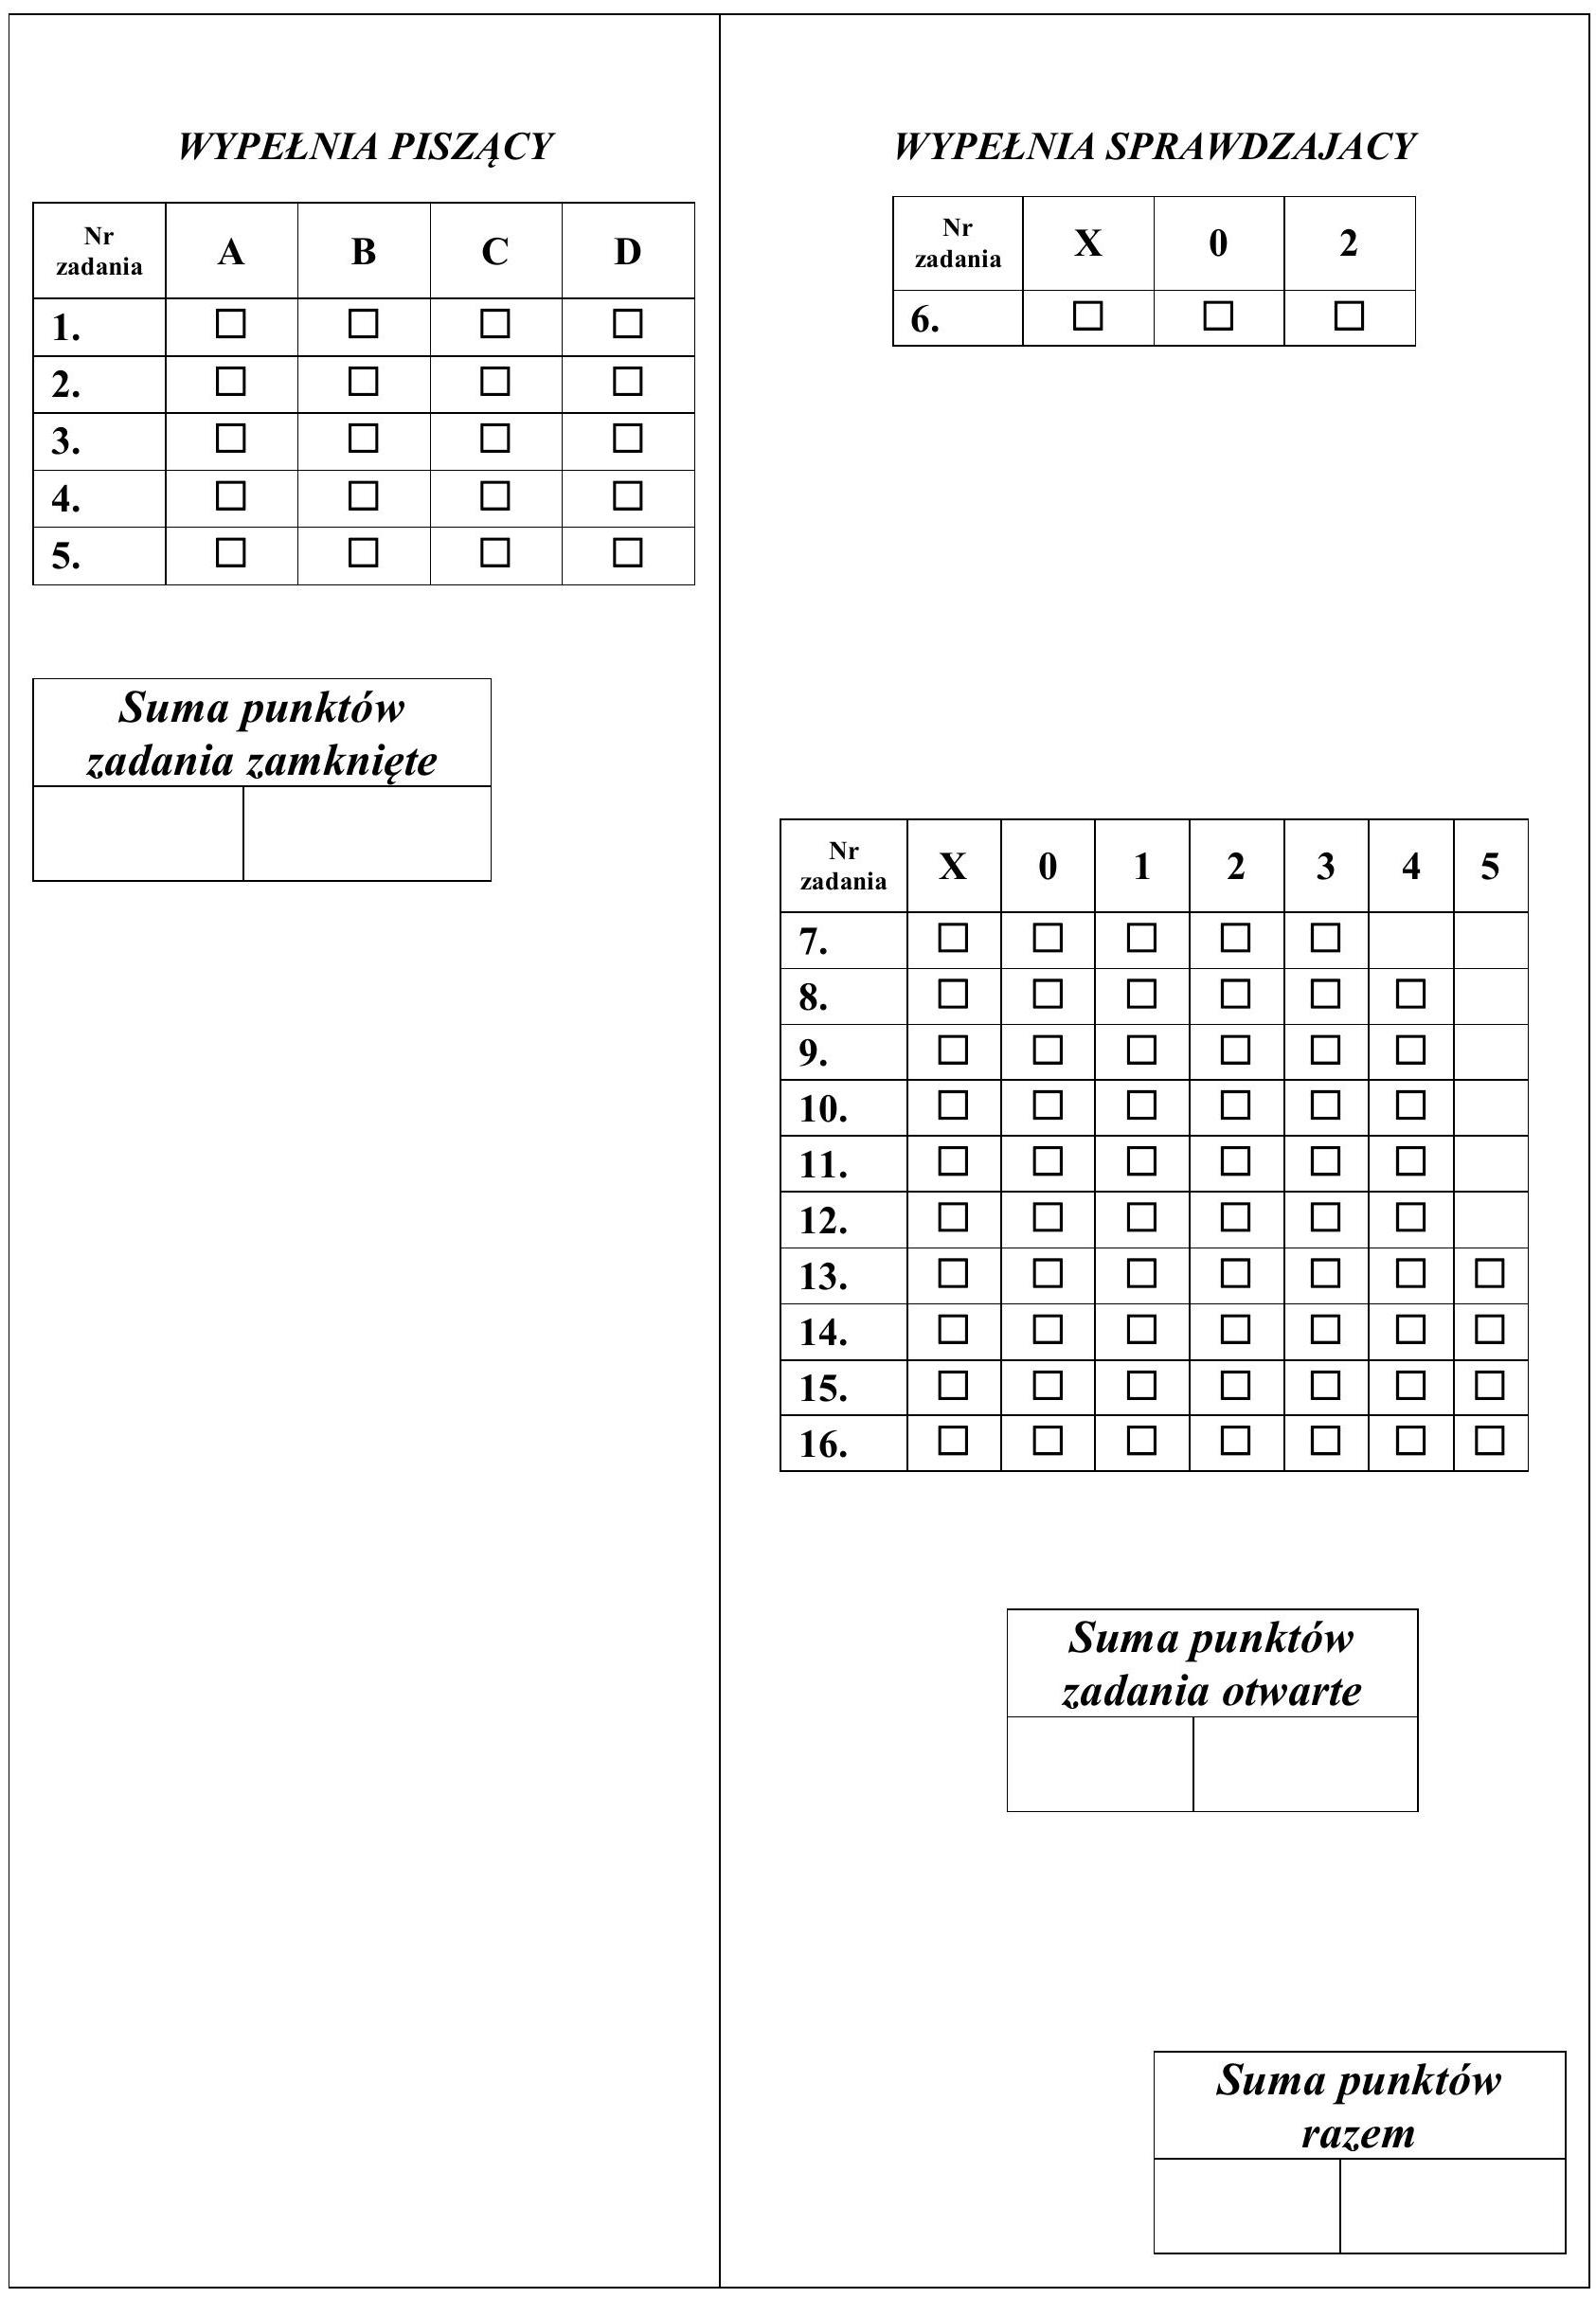
\includegraphics[max width=\textwidth, center]{2024_11_21_12a27a32a51fef2c834ag-16}


\end{document}